\chapter{Causal Models}
As you have undoubtedly heard many times in statistics classes, “correlation is
not causation.” A mere association between two variables does not necessarily
mean that one of those variables causes the other. For this reason, the
\textbf{randomized controlled experiment} is considered the standard of statistics.

We can define a randomized controlled experiment as an experiment in which all
the \textbf{factors} that influence the outcome of the experiment are either
static, or vary at random, except for one. This implies that any change in the
outcome variable must be due to that one input variable, so we can control a factor
and study how the outcome changes. This type of experiments allows us to find causal 
relationships, so we can answer to causal queries.

In cases where randomized controlled experiments are not practical, researchers
instead perform \textbf{observational studies}, in which they merely record data,
rather than controlling it. In these cases, the problem is that is difficult to
untangle the effects of different variables.

We can summarize the difference between these two types of studies as follows:
\begin{itemize}
      \item \textbf{Intervening}: we change the system assigning values to the a
            variable and observing the effect on the other variables. When we
            intervene to fix the value of a variable, we curtail the natural
            tendency of that variable to vary in response to other variables in
            nature. This amounts to performing a surgery on the graphical model,
            which we do by removing all edges directed into that variable.
            Intervening would be to take the whole population and give everyone
            treatment. This is possible if we can control the experiment, because 
            we can apply a treatment to the entire population.
      \item \textbf{Conditioning}: we merely narrow our focus to the subset of
            cases in which the variable takes the value we are interested in.
            So, conditioning on $X = x$ just means that we are restricting our
            focus to the subset of the population to those who received treatment.
\end{itemize}
We denote intervention with the \textbf{do-operator} $do(X=x)$. So, if we have
an expression which contains the do-operator, we know that we are intervening
on that variable and we call this expression a \textbf{interventional expression}.
When do do-operator doesn't appear in the expression so the expression is called 
\textbf{observational}.

An \textbf{interventional expression} which can be reduced to an \textbf{observational expression}
is said to be \textbf{identifiable}. This means that we can estimate the effect
of the intervention from the observational data.

An \textbf{estimand} is said to be:
\begin{itemize}
      \item \textbf{causal}: it contains the do-operator
      \item \textbf{statistical}: it doesn't contain the do-operator
\end{itemize}

Whenever, $do(x)$ appears in expression after the conditioning bar, it means
that everything in that expression is in the \textbf{post-intervention world}
where intervention $do(x)$ occurs.


\section{Adjustment Formula}
We can define a \textbf{causal mechanism} as a mechanism that generates $X_i$ as
the conditional distribution of $X_i$ given its parents (causes) $pa(X_i)$.

Also, we want to show that intervention are local. This means that intervening on
a variable $X_i$ only changes the causal mechanism for $X_i$; it does not change
the causal mechanisms that generate any other variables $X_j$.
\begin{definition}[\textbf{Modularity - indipendent mechanism - invariance of Causal Models}]
      If we intervene on a set of nodes $S$, setting them to constants, then for
      all $X_i \in \{X_1, \ldots, X_n\}$ we have the following:
      \begin{itemize}
            \item If $X_i \notin S$ then the causal mechanism that generates $X_i$
                  is unchanged by the intervention.
            \item If $X_i \in S$ then the causal mechanism that generates $X_i$ is
                  replaced by a constant. In other words, $P(X_i | pa(X_i)) = 1$
                  if $x$ is the value that $X_i$ is set to by the intervention
                  $do(X_i = x)$. Otherwise, we have $P(X_i | pa(X_i)) = 0$.
      \end{itemize}
\end{definition}
\begin{note}
      The \textbf{causal graph} for \textbf{interventional (experimental) distributions} is simply
      the same graph that was used for the observational joint distribution, but
      with all of the edges to the intervened node(s) removed.
\end{note}
Using do-expressions and graph surgery, we can begin to untangle the causal
relationships from the purely associative.


Not always modularity is statisfied, for example when we apply $do(X_1=x)$ 
and at the same time $P(X_4=x|X_3)$ changes, in this example modularity wasn't
fulfilled. In the reality this happens when we have hidden factor, so we 
should investigate on this factor to remove it.

\begin{note}
      It is worth noting here that we are making a tacit assumption that
      the \textbf{intervention} has no side effects. This means that applying intervention 
      this never change values for other variables.
\end{note}

The intervention procedure, which led to the \textbf{Adjustment Formula},
dictates that $Z$ should coincide with the parents $pa(X)$ of $X$, because it is
the influence of these parents that we neutralize when we fix $X$ by external
manipulation $do(X)$, so we are blocking the association path between X and Y througth
Z, setting Z.

We can therefore write a general Adjustment Formula on a set of variables and summarize it in a rule:
\begin{definition}[\textbf{Causal effect rule}]
      Given a graph $G$ in which a set of variables $pa(X)$ are designed as the
      parents of a set of variables $X$, the \textbf{causal effect} of $X$ on $Y$ can be computed
      as follows:
      \begin{equation}
            P(Y = y| do(X = x)) = \sum_{u} P(Y | X = x, pa(X) = u)P(pa(X) = u)
      \end{equation}
      where $u$ ranges over all the combinations of values that the variables in
      $pa(X)$ can take, so we are adjusting for Z or controlling for Z.
\end{definition}

So we will start from \textbf{causal estimand} $P(Y=y|do(X=x))$ and for the causal effect
rule we arrive to the \textbf{statistical estimand} which is  $\sum_z P(Y=y|X=x, Z=z) P(Z=z)$ after 
the inverversion on X. This is possible if and only if modularity is satisfied.

If we apply some manipulation on the formula, we can obtain a more convenient
form that is equivalent beacause we are moltiplying and dividing by the same quantity:
\begin{equation}
      P(Y = y| do(X = x)) = \frac{\sum_{u} P(Y = y, X = x, pa(X) = u)P(pa(X) = u)}{P(X = x | pa(X) = u)}
\end{equation}
In the equation above, the denominator $P(X = x | pa(X) = u)$ represents the \textbf{propensity score}
which displays the role played by the parents $pa(X)$ of $X$ in determining the
result of the intervention $do(X = x)$.

\section{Truncated Factorization}
In some circumstances, we can involve multiple interventions in the same time.

The previous consideration also allows us to generalize the Adjustment Formula to
\textbf{multiple intervansions}, that is, interventions that fix the values of a
set of variables $S$ to constants $s$. We simply write down the Factorization of
the pre-intervention distribution and strike out all factors that correspond to
variables in the intervention set $S$.

\begin{definition}[\textbf{Truncated Factorization (G-formula)}]
      We assume that $P$ and $G$ satisfy the Markov assumption and modularity.
      Given, a set of intervention nodes $S$, if $x_i$ is consistent with the
      intervention $S = s$, then:
      \begin{equation}
            P(x_1, x_2, \dots, x_n| do(S = s)) = \prod_{X_i\not \in S}^{n} P(X_i = x_i | pa(X_i))
      \end{equation}
      otherwise $P(x_1, x_2, \dots, x_n| do(S = s)) = 0$.
\end{definition}

\begin{note}
      Remember that pre-intervention distribution of a graph G is defined by the 
      Bayesian Network Factorization as follow:
      $$P(X_1 = x_1, X_2=x_2, \dots, X_n=x_n) = \prod_{i=1}^{n} P(X_i=x_i | pa(X_i))$$
      While the post-intervention distribution of a graph G with an intervention of 
      $S=s$ is defined as followed:
      $$P(X_1 = x_1, X_2=x_2, \dots, X_n=x_n | do(S=s)) = \prod_{X_i\not \in S}^{n} P(X_i=x_i | pa(X_i))$$
      And there is a relationship between them that is defined by:
      $$P(X_1 = x_1, X_2=x_2, \dots, X_n=x_n | do(S=s)) = \frac{P(X_1 = x_1, X_2=x_2, \dots, X_n=x_n)}{P(S=s | pa(S))}$$
      And $P(S=s | pa(S))$ is the \textbf{propensity score}.
\end{note}

Not always in every condition we can use the \textbf{causal effect rule}, infact,
in the graph represented below we have \textbf{unmeasured parents} that impact on
$X$ and $Y$, also known as
\textbf{latent}, that, though represented in the graph, may be inaccessible for
measurement. In those case, we can't adjust on each values of $pa(X)$ because we 
can't measure so we need to find an alternative set of variables to adjust for.

\begin{figure}[h]
      \centering
      \includegraphics*[width=0.7\textwidth]{img/unmeasured_parents.png}
\end{figure}

\begin{center}
      Under what conditions, is the structure of the causal graph sufficient for
      computing a causal effect from a given data set?
\end{center}

We have decided to represent causal stories with graphs so the solution becomes a graph theretical 
solution.

One of the most important tools we use to determine whether we can compute a
causal effect is a simple test called the \textbf{backdoor criterion}. Using it,
we can determine, for any two variables $X$ and $Y$ in a causal model represented
by a DAG $G$, which set of variables $S$ in that model should be conditioned on
when searching for the causal relationship between $X$ and $Y$.

\begin{definition}[\textbf{Backdoor criterion}]
      Given an ordered pair of variables $(X, Y)$ in a DAG $G$, a set of variables
      $S$ satisfies the backdoor criterion relative to $(X, Y)$ if no nodes
      in $S$ are descendants of $X$ and $S$ blocks all backdoor paths between $X$
      and $Y$ that contain an arrow into $X$.

\end{definition}
\begin{definition}[\textbf{Backdoor paths}]
      A Backdoor path is a path from $X$ to $Y$ is when there is an entering arrow in $X$.
\end{definition}

\begin{definition}[\textbf{Backdoor adjustment}]
      
      If a set of variables $S$ satisfies the backdoor criterion relative for $X$ and
      $Y$, and positivity, then the causal effect of $X$ on $Y$ is given by the following new version 
      of adjusted formula:
      \begin{equation}
            P(Y = y| do(X = x)) = \sum_{s} P(Y = y| X = x, S = s)P(S = s)
      \end{equation}
      just as when we adjust for the parents of $X$ in the Adjustment Formula. 
\end{definition}


\begin{note}
      $pa(X)$ satisfied backdoor criterion.
\end{note}

In general, we would like to condition on a set of nodes $S$ such that we:
\begin{itemize}
      \item Block all the spurious paths between $X$ and $Y$. We want the
            conditioning set $S$ to block any \textbf{backdoor path} in which
            one end has an arrow into $X$, because such paths may make $X$ and
            $Y$ dependent. (confounding effect)
      \item Leave all directed paths from $X$ to $Y$ unchanged. We don't want
            to condition on any nodes that are descendants of $X$.
      \item Create no spurious paths
\end{itemize}
\begin{figure}[!ht]
      \centering
      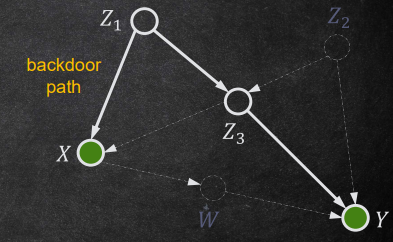
\includegraphics[width=\textwidth]{img/backdoor.png}
      \caption{Backdoor paths}
      \label{fig:backdoor}
\end{figure}
\begin{definition}[\textbf{Backdoor Adjustment Formula}]
      Give the modularity assumption, that, $S$ satisfies the backdoor criterion,
      and positivity, we can identify the causal effect of $X$ on $Y$ as follows:
      \begin{equation}
            P(Y = y| do(X = x)) = \sum_{s} P(Y = y| X = x, S = s)P(S = s)
      \end{equation}
\end{definition}

We can use the backdoor adjustment formula if, $S$ d-separates $X$ from $Y$ in
the augmented graph obtained by removing all outgoing edges from $X$. 

We would be able to isolate the causal association if $X$ is d-separated from 
$Y$ in the augmented graph.
\begin{center}
      \textbf{Isolation of the causal association is identification}
\end{center}

We can also isolate the causal association if $X$ is d-separated from $Y$ in
the augmented graph, conditional on $S$. This is what the first part of the 
backdoor criterion is about and what we've codified in the backdoor adjustment.